\section{Application Implementations}
\label{appendix:appl-impl}

Below we provide details about how we implement our applications, including the
libraries we use and how we integrate them into \sysname{}.

\para{Pedestrian Detection.} This application analyzes streams of videos from
installed CCTV cameras and detects pedestrians inside. We implement
image-related operations with OpenCV 3.1~\cite{opencvlibrary} and detect
pedestrians using histogram of oriented gradients
(HOG)~\cite{dalal2005histograms} with the default linear SVM classifier. To
ensure real-time processing of frames, we use the GPU-accelerated
implementation. Video encoding employs H.264 because of its prevalence in
existing systems. Our implementation uses GStreamer~\cite{gstreamer} with
\texttt{x264enc} plugin. To integrate with \sysname{}, we first create a
pipeline that exposes \texttt{appsrc} (to feed raw image data) and
\texttt{appsink} (to get encoded bytes). The GStreamer main loop executes in a
separate thread and \sysname{} communicates with it via Rust's channel. The
\texttt{x264enc} uses the \texttt{zerolatency} preset and four threads. We use
constant quality encoding and expose the quantization factor as another knob (in
addition to image resolution and frame rate).

Pedestrian detection returns a list of bounding boxes, and each box is a
rectangle with normalized coordinates on the image. We compare the detection
against the reference result from raw data, and declare it success if the
intersection over union (IOU) is greater than
50\%~\cite{everingham2010pascal}. We use F1 score
(\%)~\cite{Rijsbergen:1979:IR:539927} as the accuracy function and MOT16
dataset~\cite{milan2016mot16} for training and testing.

\para{Augmented Reality.} We target mobile augmented reality applications that
recognizes objects by offloading the heavy computation to resources elsewhere.
We use a similar setup (OpenCV and GStreamer) as the pedestrian detection except
for the analytical function. To recognize objects, we use YOLO~\cite{darknet13,
redmon2016yolo9000}, a GPU-enabled pre-trained neural network for object
detection. In this case, a successful detection requires matching the object
type in addition to IOU criteria. In terms of dataset, we've collected our own
video clips: the training data is a 24-second long video of an office
environment; the test data is a 246-second long video of a home environment.

\para{Distributed Top-K.} Many monitoring applications need to answer the
\textit{Top-K} question~\cite{babcock2003distributed}, such as the Top-K most
popular URLs, or the Top-K most access files. A distributed Top-K application
aggregates information from geo-distributed servers to computer a final Top-K
(\autoref{fig:topk}).

\begin{figure}
  \centering
  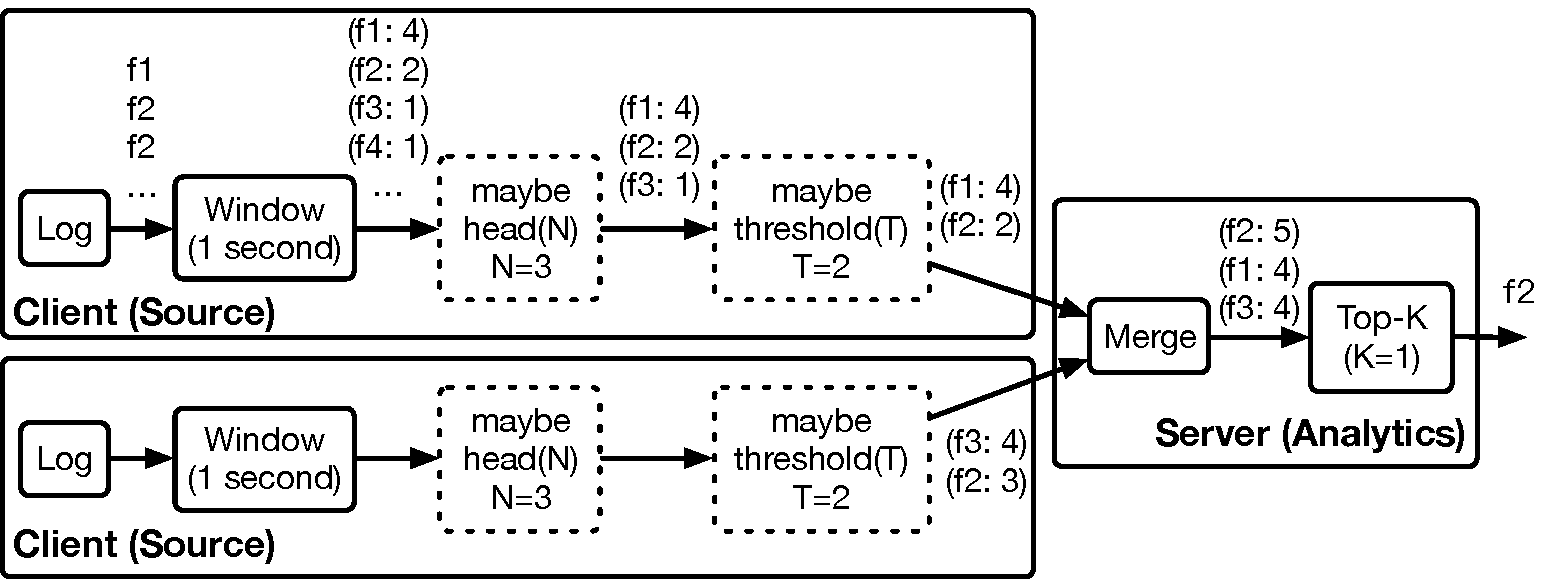
\includegraphics[width=\columnwidth]{figures/topk.pdf}
  \caption{A distributed Top-K application with two degradation operations:
    \texttt{head} and \texttt{threshold}.}
  \label{fig:topk}
\end{figure}

Naively aggregating all the raw logs is not feasible because popular servers
have millions of requests per second. Edge nodes can first perform a
\texttt{Window} operation to generate data summary, such as key-value pairs of
\texttt{<item, count>}. Even after this operation, however, the data size can
still be too large because most real-world access patterns follow a long tail
distribution. There is a large-but-irrelevant tail that contributes little to
the final results.

The edge nodes perform two degradation operations: (1) a head (\texttt{N})
operation that only takes the top \texttt{N} entries; (2) a threshold \texttt{T}
that filters small entries. These two operations are not orthogonal. Their impact on data size reduction and quality degradation depends on
the data distribution. For the accuracy function, we use Kendall's~$\tau$~\cite{abdi2007kendall}, a correlation measure of the
concordance between two ranked list. The output ranges from \(-1\) to 1,
representing no agreement to complete agreement. To integrate with \sysname{},
we convert Kendall's~$\tau$ to the range of [0, 1] with a linear transformation.

Our Top-K application aims to find the fifty most accessed files from web server
logs. We use Apache log files that record and store user access statistics for
the \href{https://www.sec.gov}{SEC.gov} website. We split these logs into four
groups, simulating four geo-distributed nodes monitoring web accesses.
To match the load of popular web servers, we compress one hour's logs into one second.

\section{Runtime Experiments}

\begin{figure}
  \centering
  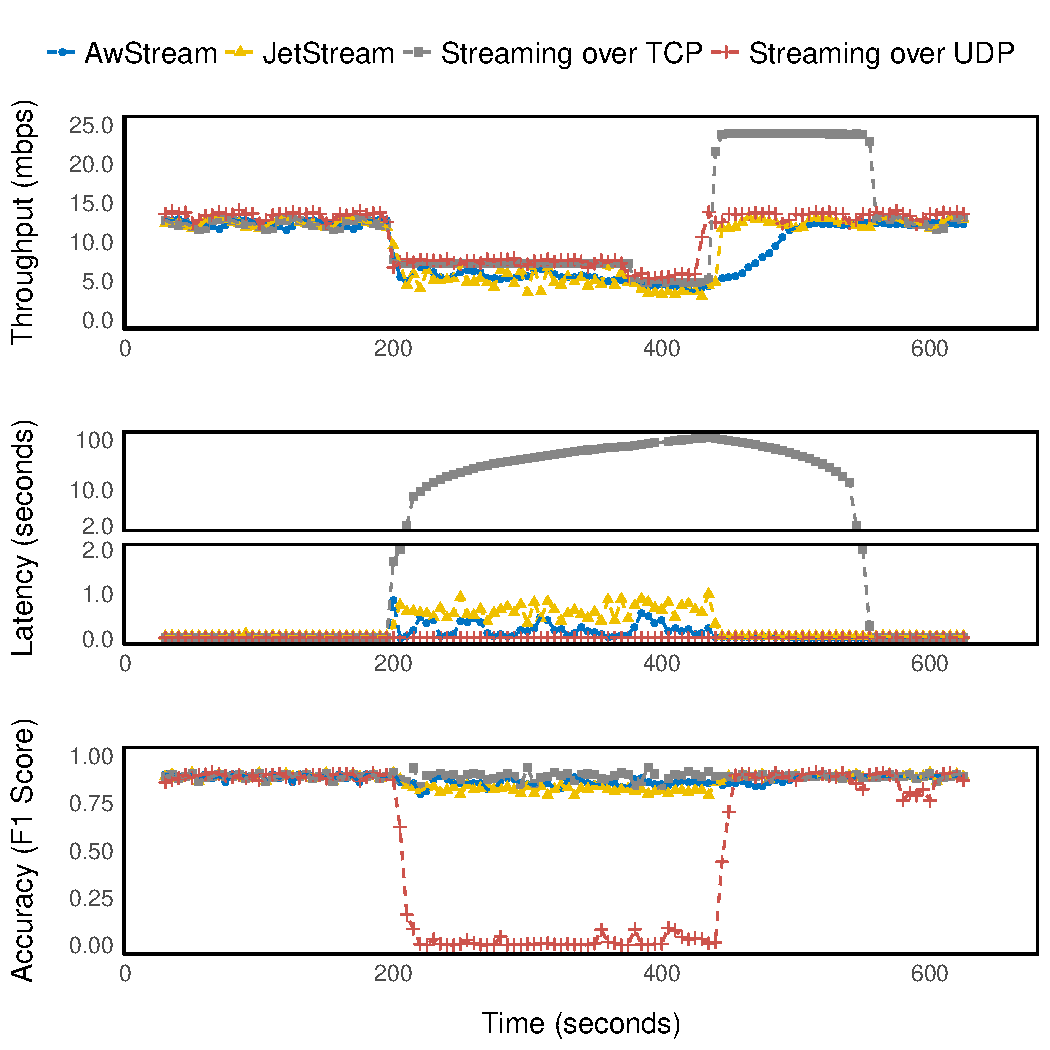
\includegraphics[width=\columnwidth]{figures/runtime-mot-verticle.pdf}
  \caption{Runtime behavior of PD application.}
  \label{fig:pd-runtime}
\end{figure}

\begin{figure}
  \centering
  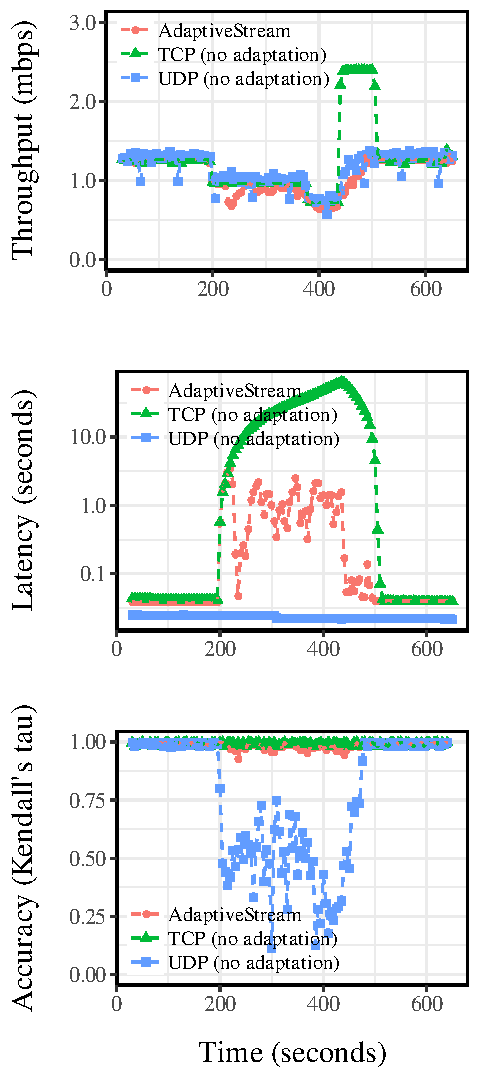
\includegraphics[width=\columnwidth]{figures/runtime-topk-verticle.pdf}
  \caption{Runtime behavior of TK application.}
  \label{fig:tk-runtime}
\end{figure}

%%% Local Variables:
%%% mode: latex
%%% TeX-master: "awstream"
%%% End:
